\documentclass[../nirs.tex]{subfiles}
\usepackage{tabularray}

\begin{document}
\section{Построение концептуальной и физической модели данных}
Основываясь на вышеперечисленные особенности разрабатываемой системы, была
создана концептуальная модель базы данных, изображенная на рисунке
\ref{fig:3_1_db_conceptual}.

\begin{figure}[H]
	\centering
	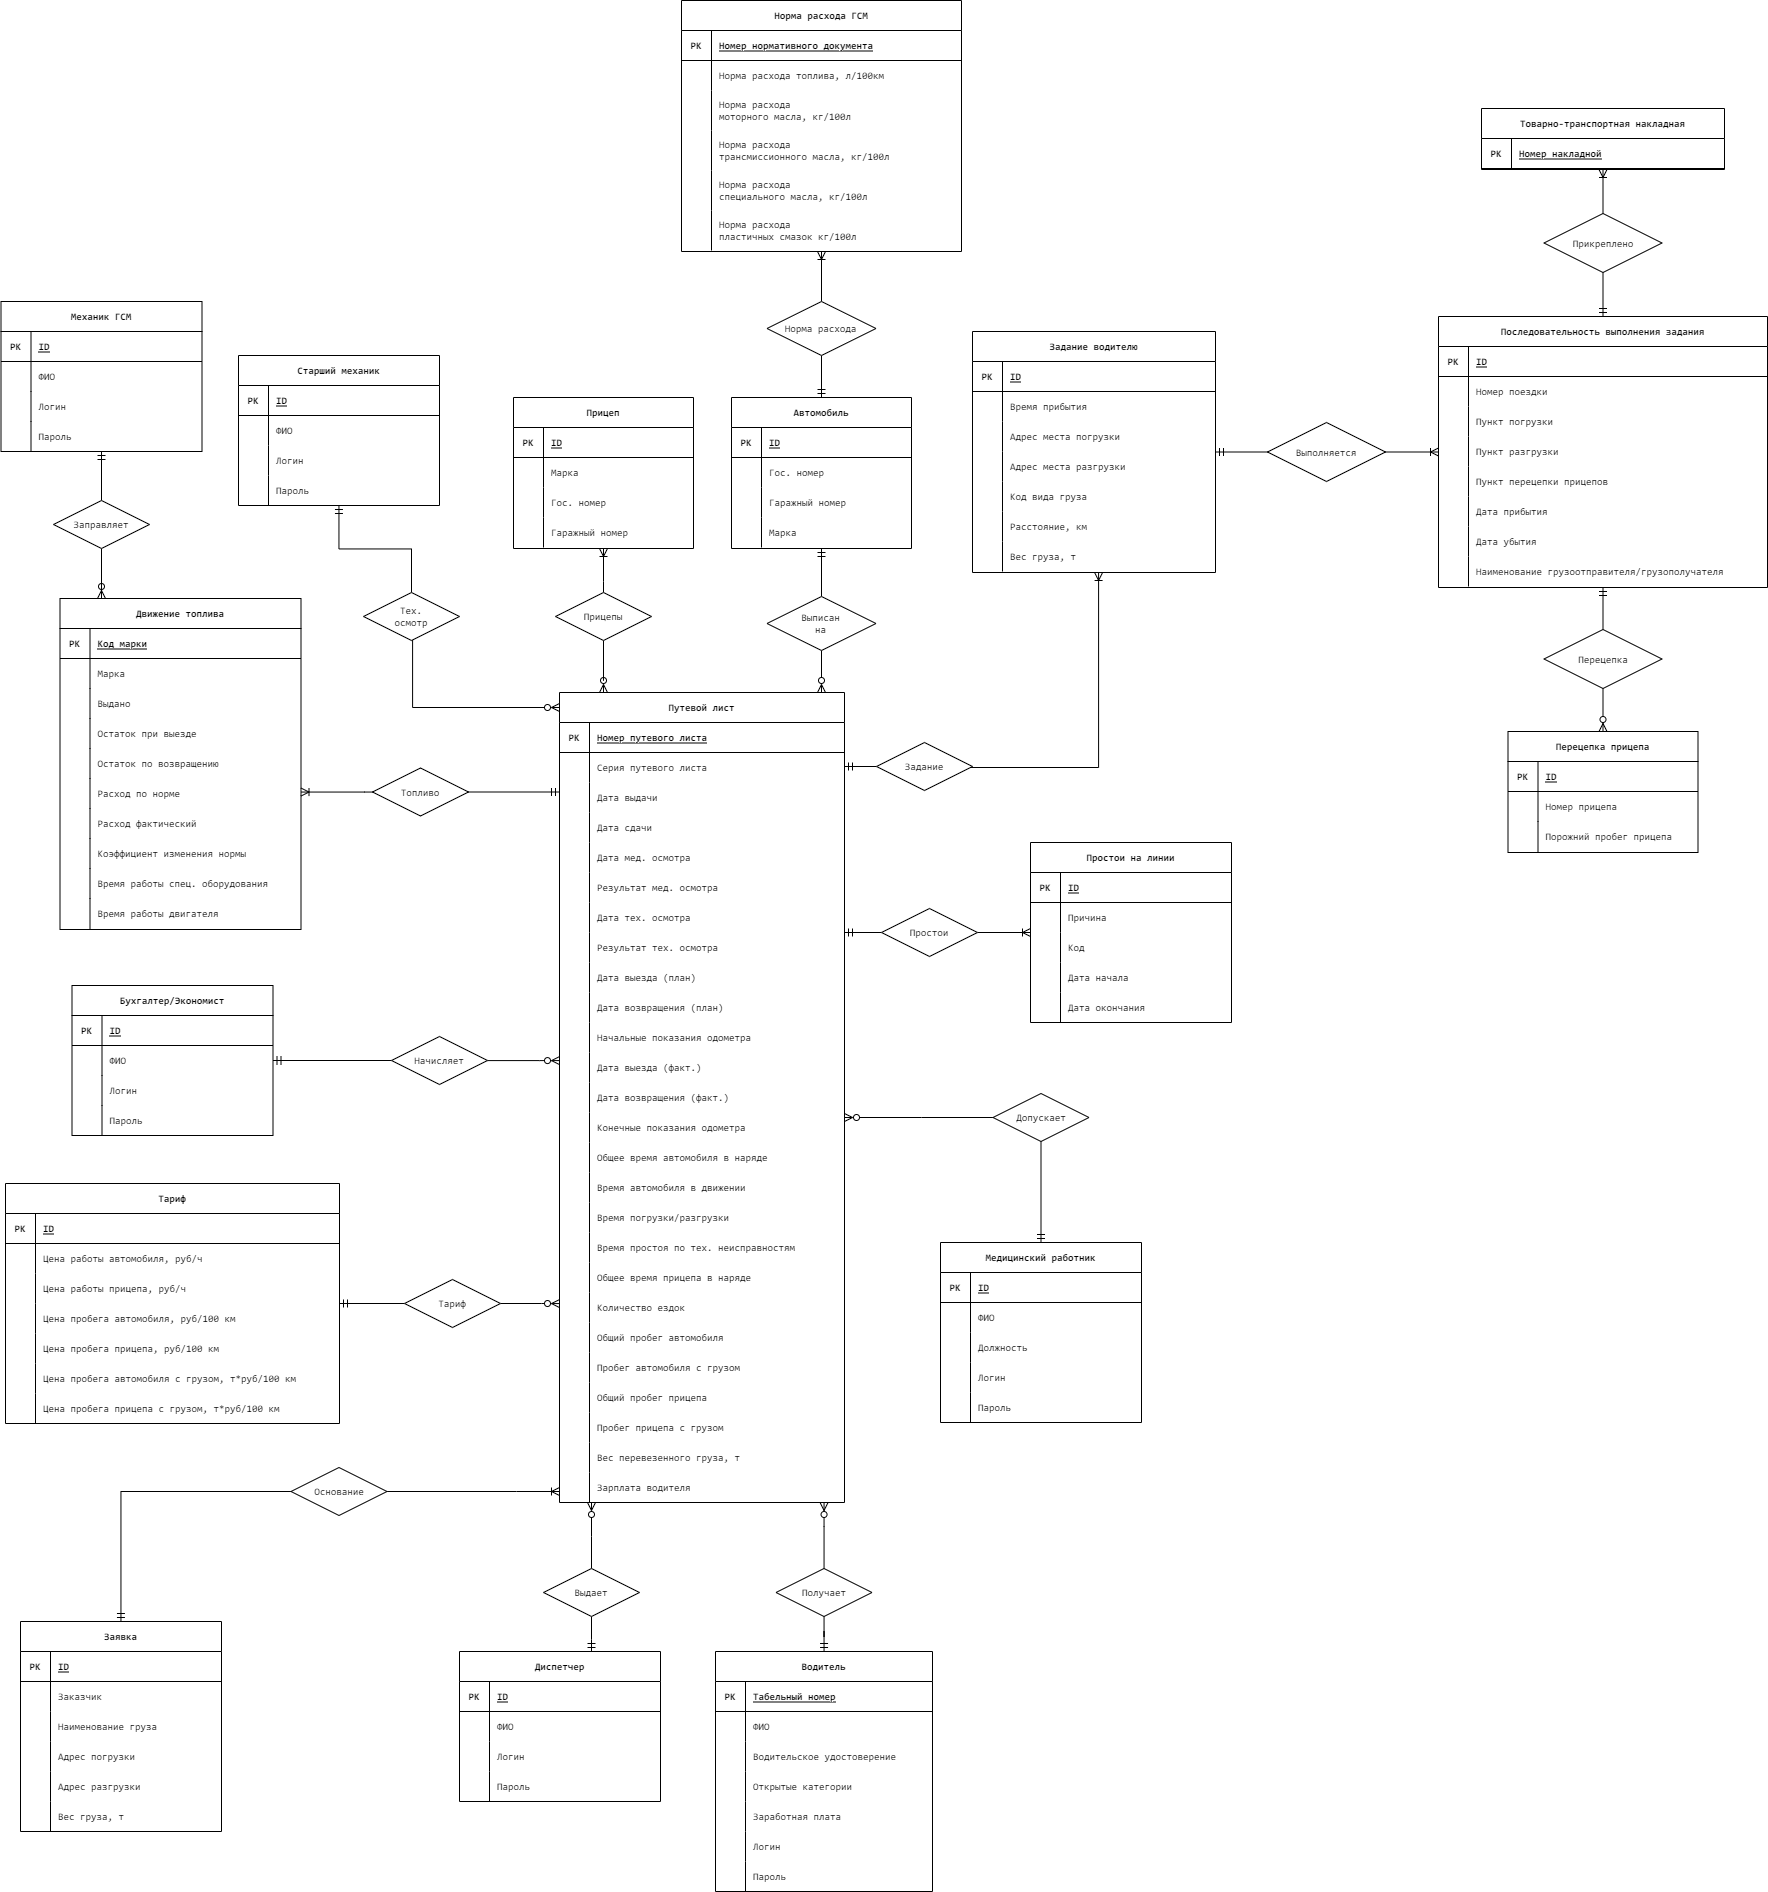
\includegraphics[keepaspectratio,width=\textwidth]{../2/images/2_1_3_er-diagram.png}
	\caption{Концептуальная модель данных разрабатываемой системы}
	\label{fig:3_1_db_conceptual}
\end{figure}

Концептуальная модель данных определяет смысловую структуру рассматриваемой
системы [8]. С ее помощью можно представить рассматриваемую предметную область
множеством сущностей и связей между ними. Каждая сущность обладает набором
свойств, именуемых атрибутами. Основная задача концептуальной модели -- передать
фундаментальное принципы и основные функциональные возможности проектируемой
системы [8].

Любая информационная система включает в себя некоторую систему управления базами
данных (СУБД). Концептуальная модель представления данных не подходит для
создания таблиц в реляционной СУБД. Чтобы можно было создать реляционную базу
данных необходимо концептуальную модель перевести в логическую, а затем в
физическую  модель данных, предназначенную для выбранной СУБД. На рисунке
\ref{fig:3_1_db_logical} представлена логическая модель данных разрабатываемой
системы.

\begin{figure}[H]
	\centering
	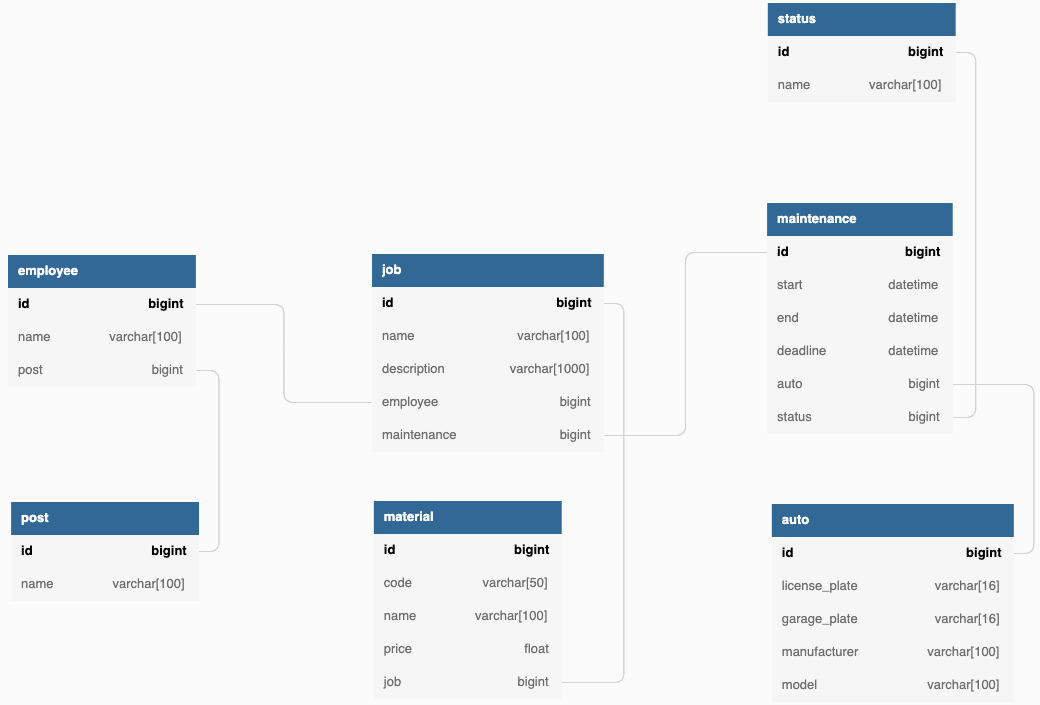
\includegraphics[keepaspectratio,width=\textwidth]{./images/3_1_db_physical.png}
	\caption{Логическая модель данных разрабатываемой системы}
	\label{fig:3_1_db_logical}
\end{figure}

Спецификация сущностей приведена в таблицах \ref{tab:waybills} --
\ref{tab:medical_workers}.
\documentclass[../1.tex]{subfiles}
\usepackage{tabularray}

\begin{document}

\begin{longtblr}
[
	caption = {Сущность \textquote{Путевой лист} (waybills)},
	label = {tab:waybills},
]
{
	hlines, vlines,
	colspec = {L c c c},
	width = \textwidth,
	rowhead = 1,
	rowfoot = 0,
}
\SetCell[c=1,r=1]{c}{Код} & Тип & M & PK \\

id & bigint & \checkmark & \checkmark \\
waybill\_number & int & \checkmark & \\
waybill\_serial & varchar(16) & & \\
waybill\_from\_date & datetime & \checkmark & \\
waybill\_expiration\_date & datetime & \checkmark & \\
waybill\_medical\_examination\_date & datetime & \checkmark & \\
waybill\_medical\_examination\_result & varchar(1024) & & \\
waybill\_maintenance\_date & datetime & \checkmark & \\
waybill\_maintenance\_result & boolean & \checkmark & \\
waybill\_checkout\_date\_planned & datetime & \checkmark & \\
waybill\_arrival\_date\_planned & datetime & \checkmark & \\
waybill\_checkout\_date & datetime & \checkmark & \\
waybill\_arrival\_date & datetime & \checkmark & \\
waybill\_odometer\_start & float & \checkmark & \\
waybill\_odometer\_end & float & \checkmark & \\
waybill\_movement\_time & timestamp & \checkmark & \\
waybill\_loading\_time & timestamp & \checkmark & \\
waybill\_failure\_time & timestamp & \checkmark & \\
waybill\_number\_of\_trips & int & \checkmark & \\
waybill\_goods\_weight & float & \checkmark & \\
auto\_mileage\_summary & float & \checkmark & \\
auto\_mileage\_with\_goods & float & \checkmark & \\
trailer\_work\_time & timestamp & \checkmark & \\
trailer\_mileage\_summary & float & \checkmark & \\
trailer\_mileage\_with\_goods & float & \checkmark & \\
driver\_wage & float & \checkmark & \\
driver & bigint & \checkmark & \\
dispatcher & bigint & \checkmark & \\
medical\_worker & bigint & \checkmark & \\
technician & bigint & \checkmark & \\
accountant & bigint & \checkmark & \\
auto & bigint & \checkmark & \\
price\_list & bigint & \checkmark & \\
request & bigint & \checkmark & \\
\end{longtblr}
\end{document}

\documentclass[../1.tex]{subfiles}
\usepackage{tabularray}

\begin{document}

\begin{longtblr}
[
	caption = {Сущность \textquote{Прицепы путевого листа} (waybill_trailers)},
	label = {tab:waybill_trailers},
]
{
	hlines, vlines,
	colspec = {L c c c},
	width = \textwidth,
	rowhead = 1,
	rowfoot = 0,
}
\SetCell[c=1,r=1]{c}{Код} & Тип & M & PK \\

waybill & bigint & \checkmark & \checkmark \\
trailer & bigint & \checkmark & \checkmark \\
\end{longtblr}
\end{document}

\documentclass[../1.tex]{subfiles}
\usepackage{tabularray}

\begin{document}

\begin{longtblr}
[
	caption = {Сущность \textquote{Заявка} (requests)},
	label = {tab:requests},
]
{
	hlines, vlines,
	colspec = {L c c c},
	width = \textwidth,
	rowhead = 1,
	rowfoot = 0,
}
\SetCell[c=1,r=1]{c}{Код} & Тип & M & PK \\

id bigint & \checkmark & \checkmark \\
request\_client\_name & varchar(2048) & \checkmark & \\
request\_goods\_name & varchar(1024) & \checkmark & \\
request\_address\_load & varchar(256) & \checkmark & \\
request\_address\_unload & varchar(256) & \checkmark & \\
request\_goods\_weight & float & \checkmark & \\
request\_arrival\_time & datetime & \checkmark & \\
request\_route\_length & float & \checkmark & \\

\end{longtblr}
\end{document}

\begin{longtblr}
[
	caption = {Сущность \textquote{Тариф} (price\_lists)},
	label = {tab:price_lists},
]
{
	hlines, vlines,
	colspec = {L c c c},
	width = \textwidth,
	rowhead = 1,
	rowfoot = 0,
}
\SetCell[c=1,r=1]{c}{Код} & Тип & M & PK \\

id & bigint & \checkmark & \checkmark \\
pl\_auto\_per\_hour & float & \checkmark & \\
pl\_trailer\_per\_hour & float & \checkmark & \\
pl\_auto\_per\_distance & float & \checkmark & \\
pl\_trailer\_per\_distance & float & \checkmark & \\
pl\_auto\_with\_goods\_per\_distance & float & \checkmark & \\
pl\_trailer\_with\_goods\_per\_distance & float & \checkmark & \\

\end{longtblr}

\begin{longtblr}
[
	caption = {Сущность \textquote{Простои} (idle\_times)},
	label = {tab:idle_times},
]
{
	hlines, vlines,
	colspec = {L c c c},
	width = \textwidth,
	rowhead = 1,
	rowfoot = 0,
}
\SetCell[c=1,r=1]{c}{Код} & Тип & M & PK \\

id & bigint & \checkmark & \checkmark \\
waybill & bigint & \checkmark & \\
idle\_code & int & \checkmark & \\
idle\_start & datetime & \checkmark & \\
idle\_end & datetime & \checkmark & \\
idle\_description & varchar(1024) & & \\

\end{longtblr}

\begin{longtblr}
[
	caption = {Сущность \textquote{Движение топлива} (fuel)},
	label = {tab:fuel},
]
{
	hlines, vlines,
	colspec = {L c c c},
	width = \textwidth,
	rowhead = 1,
	rowfoot = 0,
}
\SetCell[c=1,r=1]{c}{Код} & Тип & M & PK \\

fuel\_code & bigint & \checkmark & \checkmark \\
fuel\_task\_condition & bigint & \checkmark & \\
waybill & bigint & \checkmark & \\
refueler & bigint & \checkmark & \\
fuel\_name & varchar(256) & \checkmark & \\
waybill\_fuel\_start & float & \checkmark & \\
waybill\_fuel\_filled & float & \checkmark & \\
waybill\_fuel\_end & float & \checkmark & \\
fuel\_expense\_calculated & float & \checkmark & \\
fuel\_expense\_real & float & \checkmark & \\

\end{longtblr}

\begin{longtblr}
[
	caption = {Сущность \textquote{Условия эксплуатации} (task\_conditions)},
	label = {tab:task_conditions},
]
{
	hlines, vlines,
	colspec = {L c c c},
	width = \textwidth,
	rowhead = 1,
	rowfoot = 0,
}
\SetCell[c=1,r=1]{c}{Код} & Тип & M & PK \\

id & bigint & \checkmark & \checkmark \\
condition\_altitude & float & \checkmark & \\
condition\_road\_quality & enum\_road\_category & \checkmark & \\
condition\_difficult\_route & boolean & \checkmark & \\
condition\_city\_population & float & \checkmark & \\
condition\_often\_stops & boolean & \checkmark & \\
condition\_slow\_speed & enum\_slow\_speed\_class & \checkmark & \\
condition\_auto\_run\_in & boolean & \checkmark & \\
condition\_auto\_transit & enum\_auto\_transit & \checkmark & \\
condition\_technological\_transport & boolean & \checkmark & \\
condition\_special\_transport & boolean & \checkmark & \\
condition\_work\_at\_low\_quality\_roads & boolean & \checkmark & \\
condition\_work\_emergency & boolean & \checkmark & \\
condition\_training\_driving & enum\_training\_driving & \checkmark & \\
condition\_climate\_control & boolean & \checkmark & \\
condition\_forced\_idle\_time & boolean & \checkmark & \\
condition\_warmup\_time & boolean & \checkmark & \\

\end{longtblr}

\begin{longtblr}
[
	caption = {Сущность \textquote{Автомобиль} (autos)},
	label = {tab:autos},
]
{
	hlines, vlines,
	colspec = {L c c c},
	width = \textwidth,
	rowhead = 1,
	rowfoot = 0,
}
\SetCell[c=1,r=1]{c}{Код} & Тип & M & PK \\

id & bigint & \checkmark & \checkmark \\
tech\_registration\_number & varchar(64) & \checkmark & \\
tech\_model\_name & varchar(1024) & \checkmark & \\

\end{longtblr}

\documentclass[../1.tex]{subfiles}
\usepackage{tabularray}

\begin{document}

\begin{longtblr}
[
	caption = {Сущность \textquote{Трейлер} (trailers)},
	label = {tab:trailers},
]
{
	hlines, vlines,
	colspec = {L c c c},
	width = \textwidth,
	rowhead = 1,
	rowfoot = 0,
}
\SetCell[c=1,r=1]{c}{Код} & Тип & M & PK \\

id & bigint & \checkmark & \checkmark \\
tech\_registration\_number & varchar(64) & \checkmark & \\
tech\_model\_name & varchar(1024) & \checkmark & \\

\end{longtblr}
\end{document}

\documentclass[../1.tex]{subfiles}
\usepackage{tabularray}

\begin{document}

\begin{longtblr}
[
	caption = {Сущность \textquote{Норма расхода топлива} (fuel\_wasting)},
	label = {tab:fuel_wasting},
]
{
	hlines, vlines,
	colspec = {L c c c},
	width = \textwidth,
	rowhead = 1,
	rowfoot = 0,
}
\SetCell[c=1,r=1]{c}{Код} & Тип & M & PK \\

id & bigint & \checkmark & \checkmark \\
fw\_fuel\_waste & float & \checkmark & \\
fw\_oil\_waste & float & \checkmark & \\
auto & bigint & \checkmark & \\

\end{longtblr}
\end{document}

\documentclass[../1.tex]{subfiles}
\usepackage{tabularray}

\begin{document}

\begin{longtblr}
[
	caption = {Сущность \textquote{Задание водителю} (tasks)},
	label = {tab:tasks},
]
{
	hlines, vlines,
	colspec = {L c c c},
	width = \textwidth,
	rowhead = 1,
	rowfoot = 0,
}
\SetCell[c=1,r=1]{c}{Код} & Тип & M & PK \\

id & bigint & \checkmark & \checkmark \\
request & bigint & \checkmark & \\
task\_goods\_name & varchar(1024) & \checkmark & \\
task\_address\_load & varchar(256) & \checkmark & \\
task\_address\_unload & varchar(256) & \checkmark & \\
task\_goods\_weight & float & \checkmark & \\
task\_route\_length & float & \checkmark & \\

\end{longtblr}
\end{document}

\begin{longtblr}
[
	caption = {Сущность \textquote{Выполнение задания} (task\_completions)},
	label = {tab:task_completions},
]
{
	hlines, vlines,
	colspec = {L c c c},
	width = \textwidth,
	rowhead = 1,
	rowfoot = 0,
}
\SetCell[c=1,r=1]{c}{Код} & Тип & M & PK \\

id & bigint & \checkmark & \checkmark \\
task\_trip\_number & int & \checkmark & \\
task\_departure\_address & varchar(256) & \checkmark & \\
task\_arrival\_address & varchar(256) & \checkmark & \\
task\_departure\_date & datetime & \checkmark & \\
task\_arrival\_date & datetime & \checkmark & \\
task & bigint & \checkmark & \\
trailer\_change & bigint & & \\

\end{longtblr}

\documentclass[../1.tex]{subfiles}
\usepackage{tabularray}

\begin{document}

\begin{longtblr}
[
	caption = {Сущность \textquote{Товарно-транспортная накладная}
	(consignment\_notes)},
	label = {tab:consignment_notes},
]
{
	hlines, vlines,
	colspec = {L c c c},
	width = \textwidth,
	rowhead = 1,
	rowfoot = 0,
}
\SetCell[c=1,r=1]{c}{Код} & Тип & M & PK \\

id & bigint & \checkmark & \checkmark \\
task\_completion & bigint & \checkmark & \\

\end{longtblr}
\end{document}

\begin{longtblr}
[
	caption = {Сущность \textquote{Перецепка прицепа} (trailer\_changes)},
	label = {tab:trailer_changes},
]
{
	hlines, vlines,
	colspec = {L c c c},
	width = \textwidth,
	rowhead = 1,
	rowfoot = 0,
}
\SetCell[c=1,r=1]{c}{Код} & Тип & M & PK \\

id & bigint & \checkmark & \checkmark \\
trailer & bigint & \checkmark & \\
trailer\_change\_address & varchar(256) & \checkmark & \\
trailer\_empty\_mileage & float & \checkmark & \\

\end{longtblr}

\documentclass[../1.tex]{subfiles}
\usepackage{tabularray}

\begin{document}

\begin{longtblr}
[
	caption = {Сущность \textquote{Тип пользователя} (user\_types)},
	label = {tab:user_types},
]
{
	hlines, vlines,
	colspec = {L c c c},
	width = \textwidth,
	rowhead = 1,
	rowfoot = 0,
}
\SetCell[c=1,r=1]{c}{Код} & Тип & M & PK \\

id & bigint & \checkmark & \checkmark \\
name & varchar(256) & \checkmark & \\

\end{longtblr}
\end{document}

\documentclass[../1.tex]{subfiles}
\usepackage{tabularray}

\begin{document}

\begin{longtblr}
[
	caption = {Сущность \textquote{Пользователь} (users)},
	label = {tab:users},
]
{
	hlines, vlines,
	colspec = {L c c c},
	width = \textwidth,
	rowhead = 1,
	rowfoot = 0,
}
\SetCell[c=1,r=1]{c}{Код} & Тип & M & PK \\

id & bigint & \checkmark & \checkmark \\
user\_type & bigint & \checkmark & \\
user\_name & varchar(512) & \checkmark & \\
user\_login & varchar(512) & \checkmark & \\
user\_password & varchar(512) & \checkmark & \\

\end{longtblr}
\end{document}

\documentclass[../1.tex]{subfiles}
\usepackage{tabularray}

\begin{document}

\begin{longtblr}
[
	caption = {Сущность \textquote{Водитель} (drivers)},
	label = {tab:drivers},
]
{
	hlines, vlines,
	colspec = {L c c c},
	width = \textwidth,
	rowhead = 1,
	rowfoot = 0,
}
\SetCell[c=1,r=1]{c}{Код} & Тип & M & PK \\

id & bigint & \checkmark & \checkmark \\
user & bigint & \checkmark & \\
driver\_license\_number & bigint & \checkmark & \\
driver\_license\_class & int & \checkmark & \\
driver\_wage & float & \checkmark & \\

\end{longtblr}
\end{document}

\begin{longtblr}
[
	caption = {Сущность \textquote{Медицинский работник} (medical\_workers)},
	label = {tab:medical_workers},
]
{
	hlines, vlines,
	colspec = {L c c c},
	width = \textwidth,
	rowhead = 1,
	rowfoot = 0,
}
\SetCell[c=1,r=1]{c}{Код} & Тип & M & PK \\

id & bigint & \checkmark & \checkmark \\
user & bigint & \checkmark & \\
medical\_worker\_post & varchar(256) & \checkmark & \\

\end{longtblr}


\end{document}
